\newcommand{\xbold}{{\bf x}}
\newcommand{\ebis}{{\tt EBIndexSpace}}
\newcommand{\baseif}{{\tt BaseIF}}
\newcommand{\sphereif}{{\tt SphereIF}}
\newcommand{\transformif}{{\tt TransformIF}}
\newcommand{\latheif}{{\tt LatheIF}}
\newcommand{\unionif}{{\tt UnionIF}}
\newcommand{\intersectionif}{{\tt IntersectionIF}}
\newcommand{\geom}{{\tt GeometryShop}}
\newcommand{\parm}{{\tt ParmParse}}

For computations with complex geometries, $\tt{AMReX}$ provides data
structures and iterators for performing Cartesian grid, embedded
boundary (EB) calculations.   Examples include elliptic solvers and a
compressible Navier Stokes simulation.  
The overall goals of $\tt{AMReX}$'s EB tools are to allow users 
to write simulations involving complex geomtery  without having to
rewrite the common motifs that appear in these calculations.  
We give an overview of $\tt{AMReX}$'s EB classes and how to use them.

\section{Overview of Embedded Boundary Description}
\label{sec:EB:EBOverview}

Cartesian grids with embedded boundaries are 
useful to describe
volume-of-fluid representations of irregular boundaries.
In this description,
geometry is represented by volumes ($\Lambda h^d$) and apertures 
($\vec{A}^\alpha h^{d-1}$).   See figure \ref{fig::volume}
for an illustration.  In the figure, the grey area represents 
the region excluded from the solution domain and the arrows represent
fluxes.  A conservative, ``finite volume'' discretization
of a flux divergence $\nabla \cdot \vec{F}$ is of the form:
\begin{equation}
\nabla \cdot \vec{F} \approx \frac{1}{\Lambda h} \sum \vec{F}^\alpha \cdot
\vec{A}^\alpha
\end{equation}
This is useful for many important partial differential equations.
Consider  Poisson's equation with Neumann boundary conditions
\begin{equation}
\nabla \cdot \vec{F} = \Delta \phi = \rho \hbox{ on $\Omega$ }.
\end{equation}
\begin{equation}
\frac{\partial \phi}{\partial n} = 0 \hbox{ on $\partial \Omega$}
\end{equation}
The volume-of fluid description reduces the problem to finding
sufficiently accurate gradients at the apertures.   
The only geometric information required for second order embedded
boundary algorithms are:
\begin{itemize}
\item
Volume fractions
\item
Area fractions
\item 
Centers of volume, area.
\end{itemize}
The problem with this description of the geometry 
is it can create  multiply-valued cells and
non-rectangular connectivity.
Refer to figure \ref{fig::graph}.  
The interior of the cartoon airfoil represents the area
excluded from the domain and the lines connecting the cell centers
represent the connectivity of the discrete domain
This very simple geometry produces a graph
which is more complex than a rectangular lattice simply because
the grid which surrounds it cannot resolve the geometry.
The lack of resolution is fundamental to many geometries 
of interest (trailing edges of airfoils, infinitely thin shells).
Algorithms which require grid coarsening (multigrid, for example)
also produce grids where such complex connectivity occurs.
The connectivity can become arbitrarily complex (see figure 
\ref{fig::multidivide}) in general, so the software infrastructure
must support abstractions which can express this complexity.

Our solution to this abstraction problem is to
define the embedded boundary grid as a graph.
The irregular part of the index space can be represented by a graph 
$G = \{N,E\}$, where $N$ is the set of all nodes in the graph, and 
$E$ the set of all edges of the graph connecting various pairs of 
nodes. Geometrically,
the nodes correspond to irregular control volumes (cell fragments) 
cut out by the intersection of the body with the rectangular mesh, and 
the edges correspond to the parts of cell faces that abut a pair of irregular 
cell fragments. The remaining parts of space are indexed using elements
of $Z^d$, or are covered by the body, and not indexed into at all. However,
it is possible to think of the entire index space (both the regular and
irregular parts) as a graph: in the regular part of the index space,
the nodes are just elements of $Z^d$, and the 
edges are the cell faces that
separate pair of successive cells along the coordinate directions. 


\begin{figure}
  \centering
  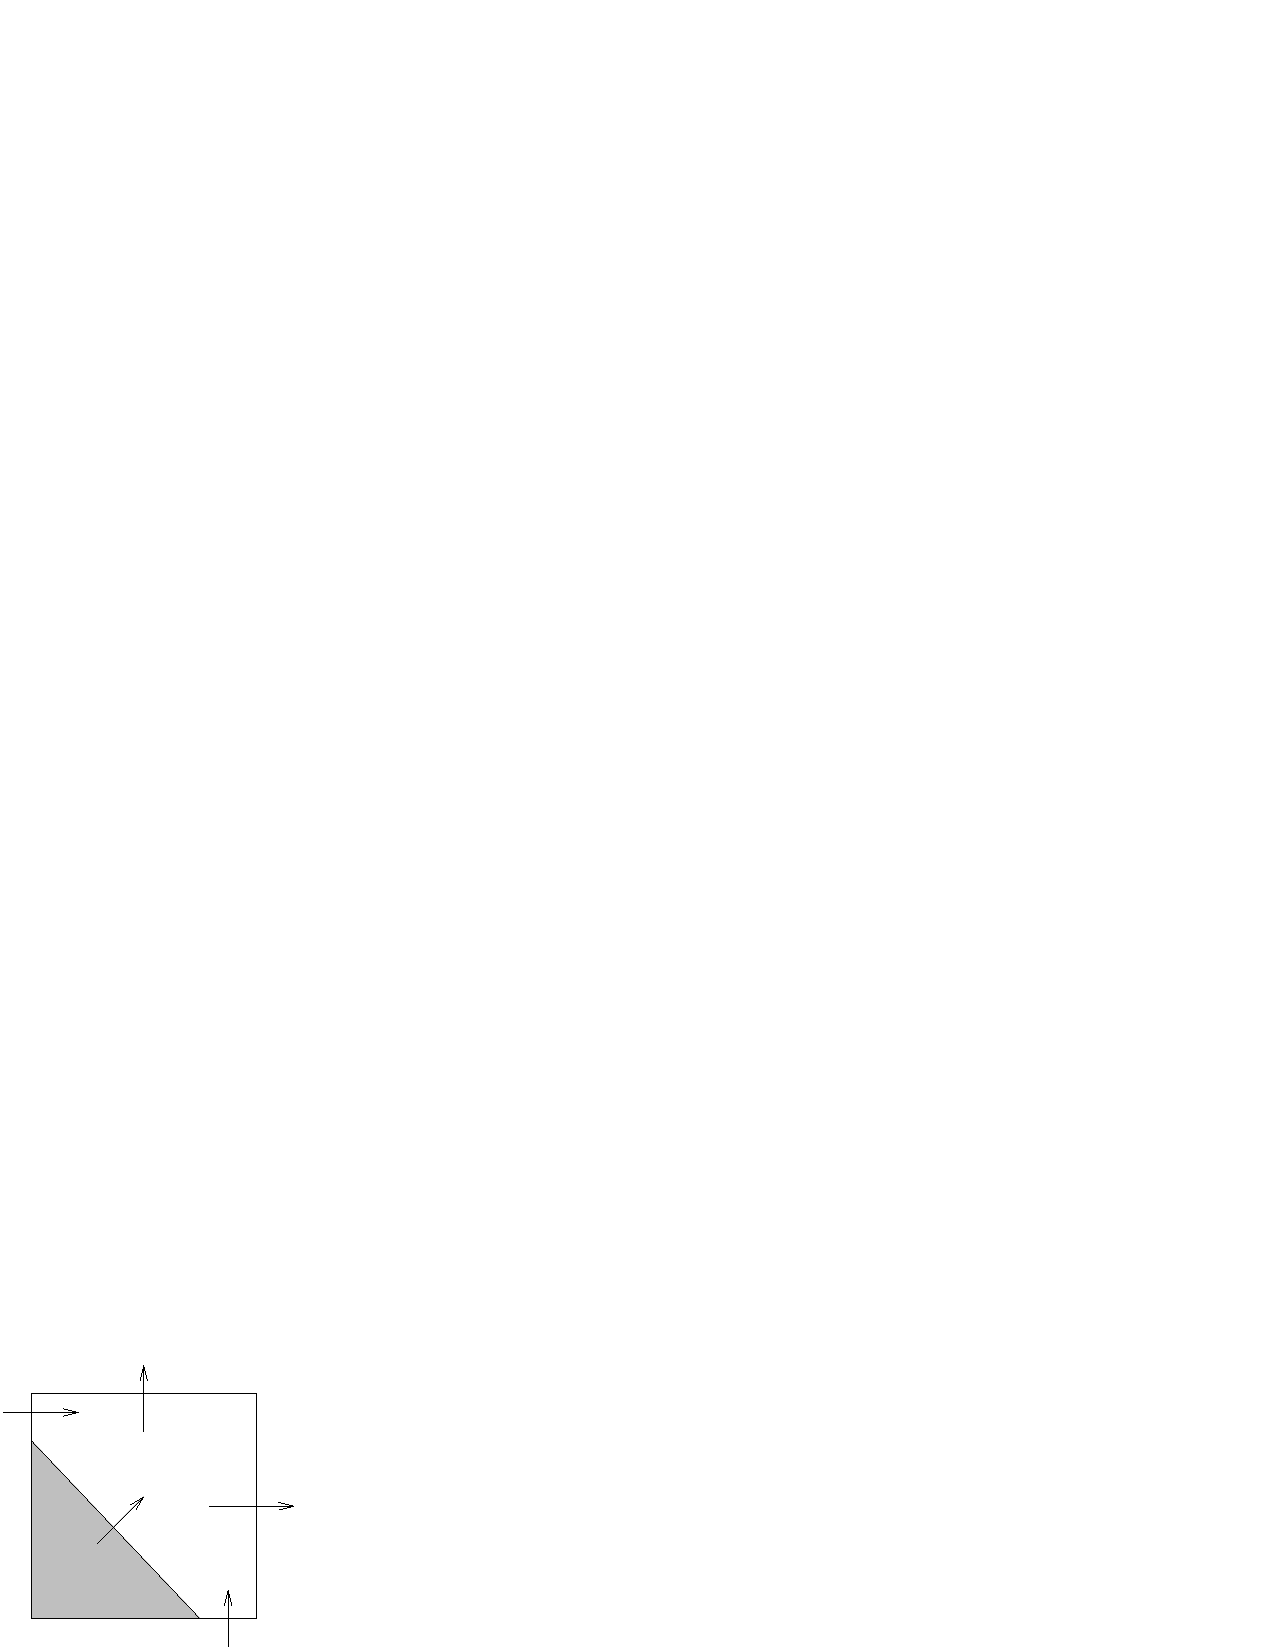
\includegraphics[width=\textwidth]{./EB/volume.pdf}
\caption{\label{fig::volume}Embedded boundary cell. The grey area represents 
the region excluded from the solution domain and the arrows represent
fluxes.}
\end{figure}

\begin{figure}
  \centering
  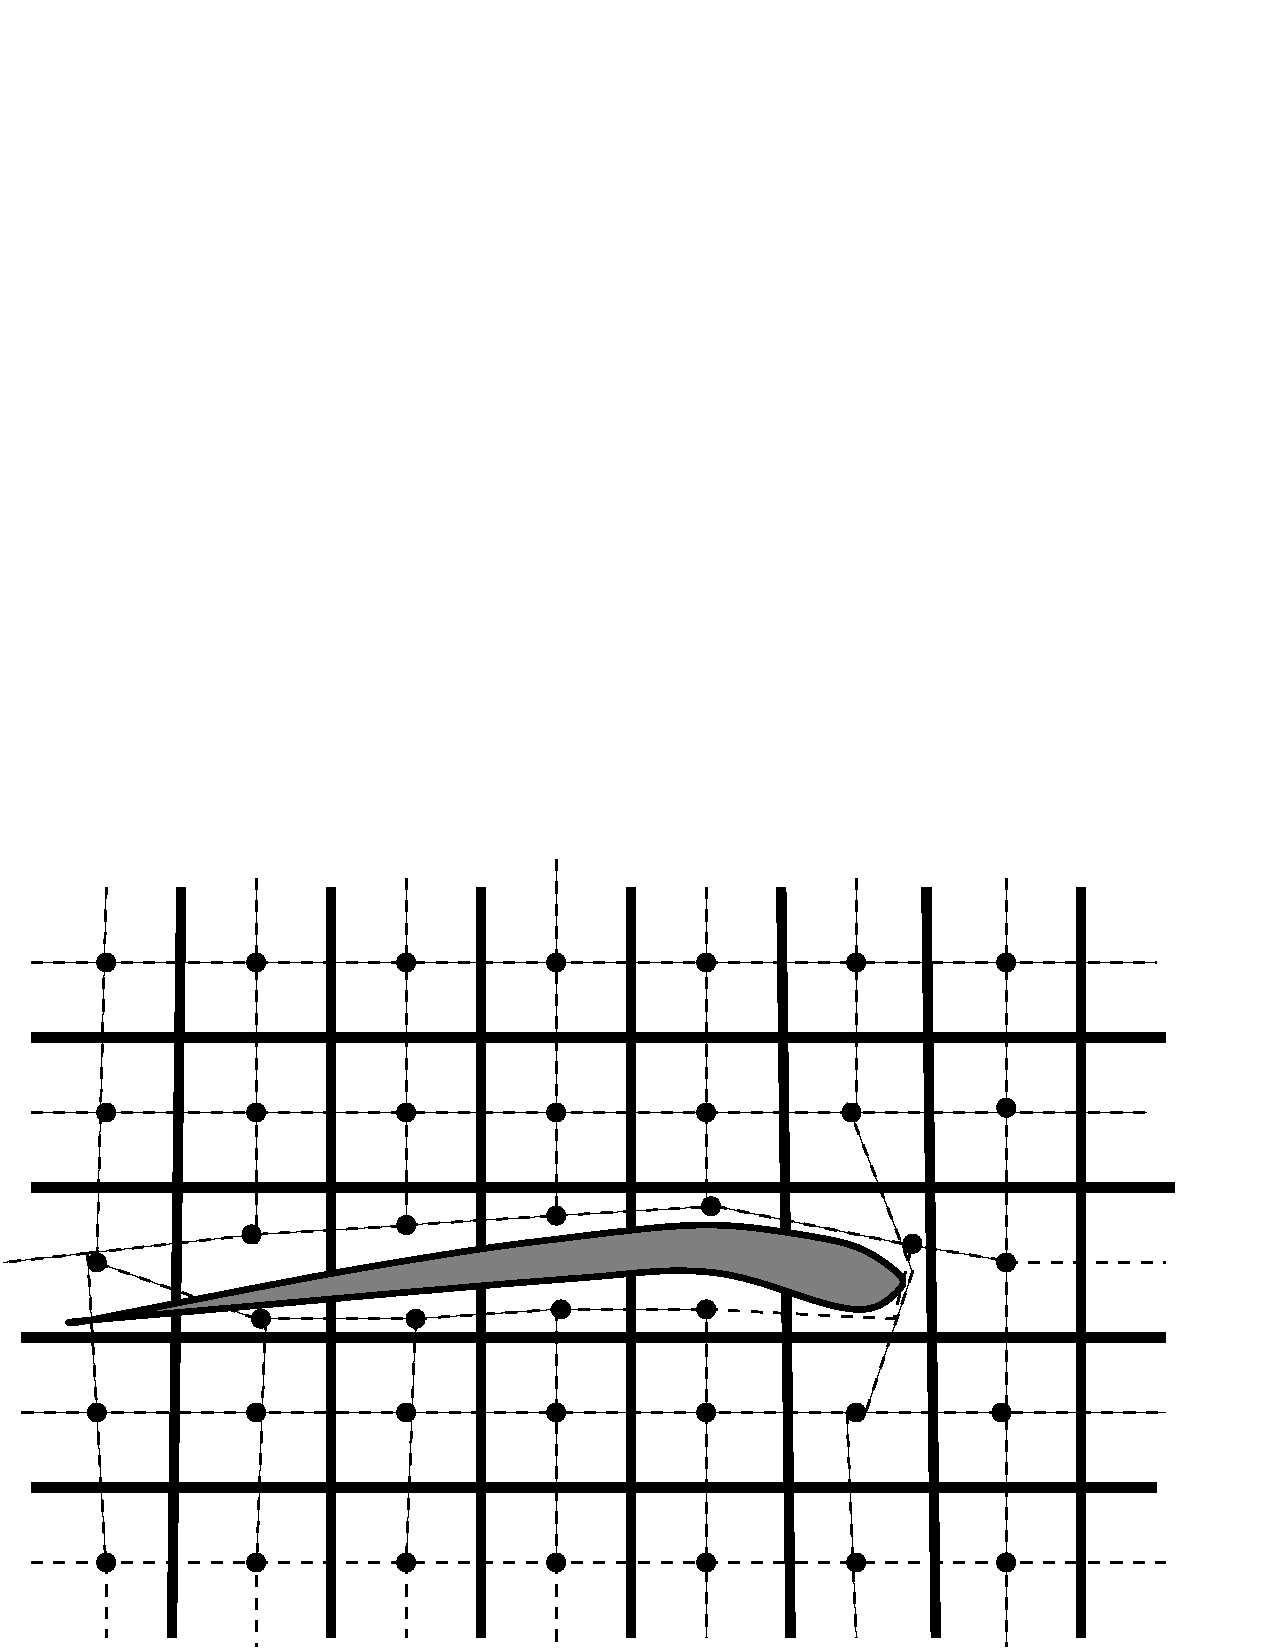
\includegraphics[width=\textwidth]{./EB/graph.pdf}
\caption{Example of embedded boundary description of an interface. 
The interior of the cartoon airfoil represents the area
excluded from the domain and the lines connecting the cell centers
represent the graph connectivity of the discrete domain.    }
\label{fig::graph}
\end{figure}

\begin{figure}
  \centering
  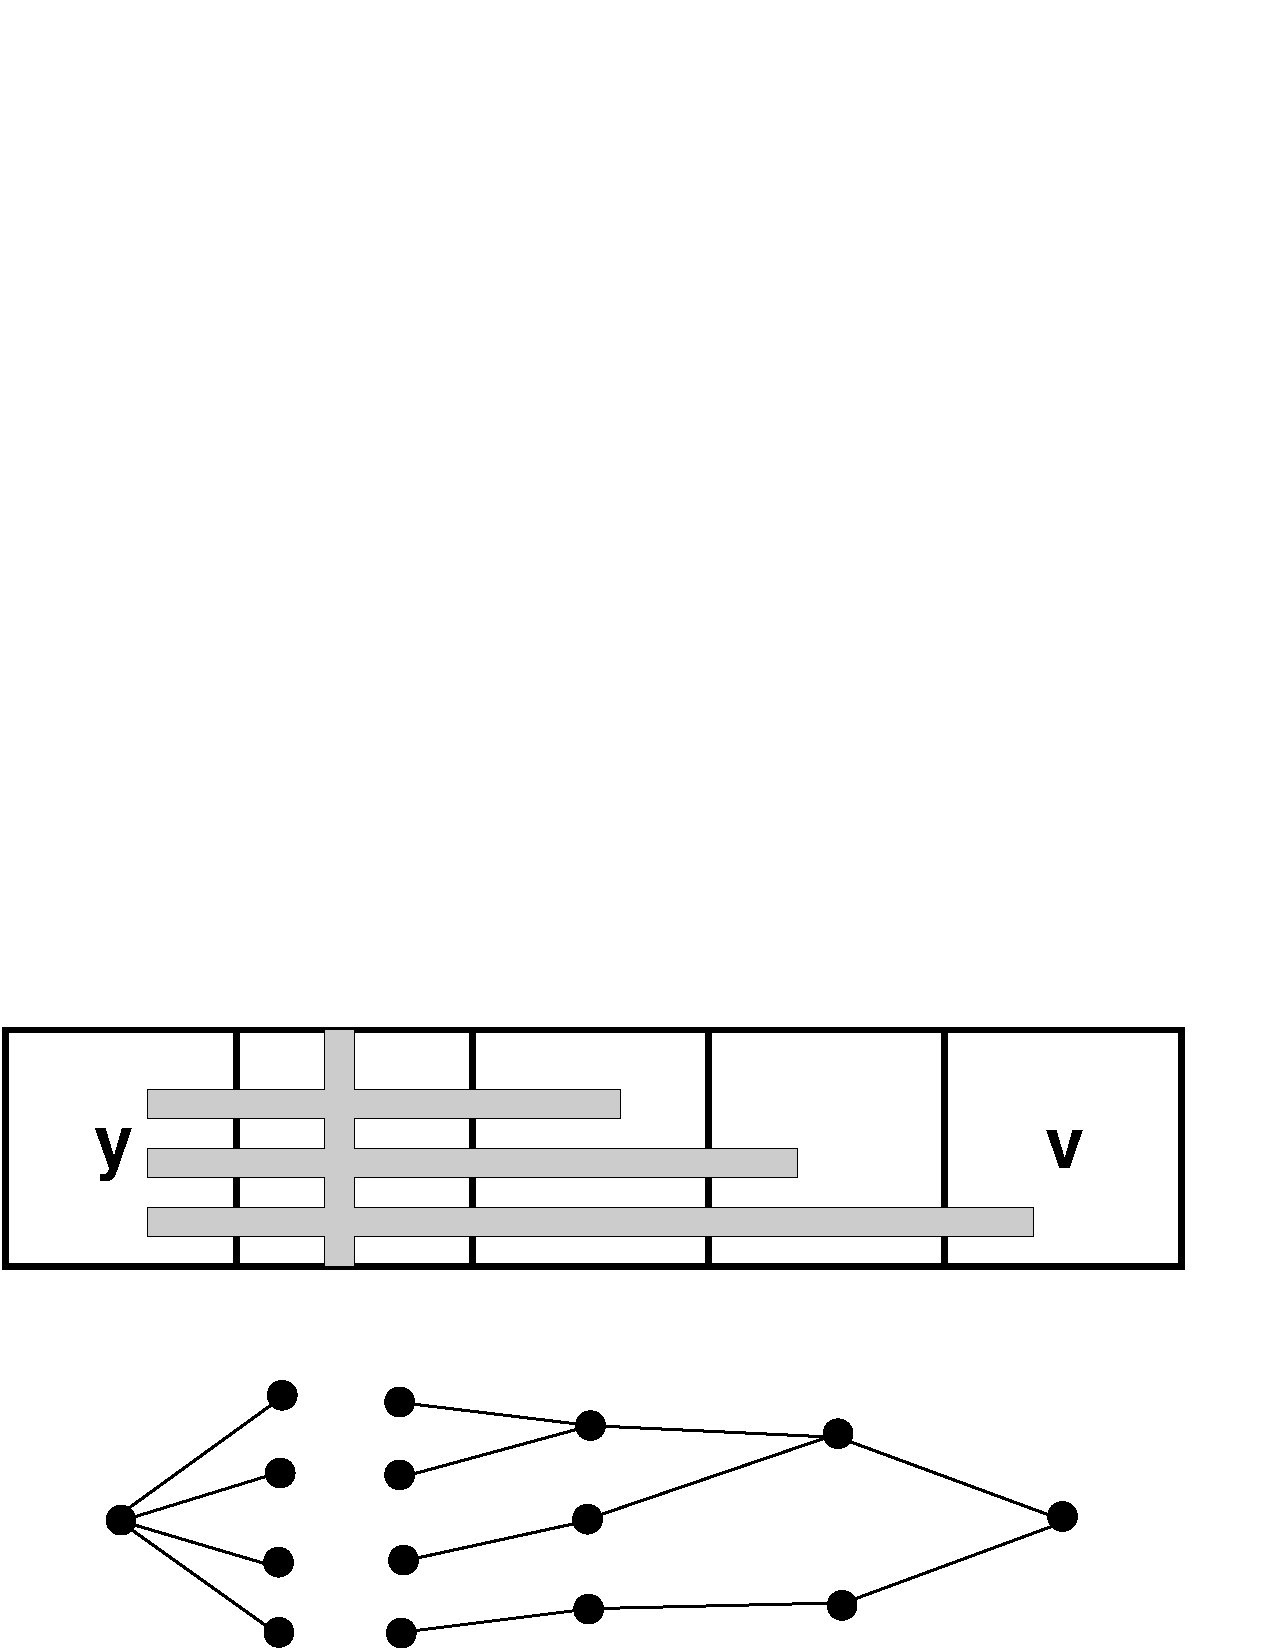
\includegraphics[width=\textwidth]{./EB/multidivide.pdf}
\caption{\label{fig::multidivide}Example of embedded boundary description of an interface
and its corresponding graph description.  The graph
can be almost arbitrarily complex when the grid is
underresolved.}
\end{figure}


\section{Initializing \ebis}
\label{sec:EB:ebinit}

This geometric information, along with its associated connectivity
graph is stored in a distributed database class \ebis which must be
initialized at the start of the calculation.    The procedure for this
goes as follows.   To initialize this database, one follows these steps:
\begin{itemize}
\item Define an implicit function which describes the surface 
      and use it define a \geom object (see \S
      \ref{sec:EB:geometryshop}).
\item Call $\tt{EBIndexSpace::define}$ with the \geom object.   This
  will fill the database of graph and moment data.   It is important
  to define this using the finest resolution of domain that will be
  used in the calculation.   Coarser information is generated
  automatically by \ebis by graph coarsening.
\end{itemize}
As an illustration, here is how one would define the \ebis where the
geometry is described as the complement of a sphere of radius 0.1
centered inside a unit cube where the maxium resolution is $1024^3$.
The classes involved are described in \S \ref{sec:EB:geometryshop}.

\begin{lstlisting}[language=cpp]

  int nx = 1024;
  Box domain(IntVect::Zero, (nx-1)*IntVect::Unit);
  Real dx = 1.0/nx;
  Real radius = 0.1;
  Real center = 0.5*RealVect::Unit;
  bool insideRegular = false;
  //this is the implicit function
  SphereIF sphere(radius, center, insideRegular);

  //this is worker object that creates geometric information given an IF
  GeometryShop workshop(sideImpMultisphere)

  //this is the global, distributed database being initialized
  EBIndexSpace*  ebis = AMReX_EBIS::instance()
  ebis->define(domain, RealVect::Zero, dx, workshop);

\end{lstlisting}

%%After this initialization is complete, any part of the calculation can
%%access the data via $\tt{EBIndexSpace::fillEBISLayout}$.

\subsection{GeometryShop and Implicit Functions}
\label{sec:EB:geometryshop}

One of the greatest advantages of EB technology is that grid
generation is robust and fast and can be done to any accuracy
The foundation class that AMReX uses for
geometry generation is called \geom.  Given an implicit
function $I$  \geom interprets the surface upon which $I(\xbold) = 0$
as the surface with which to cut the grid cells.   \geom interprets
the positive regions of the implicit function ($\xbold: I(\xbold) > 0$)
as covered by the geometry  negative regions ($\xbold: I(\xbold) < 0$) 
as part of  the solution domain.  For example, if one defines her
implicit function $S$ as
$$
S(\xbold) = x^2 + y^2 + z^2 - R^2,
$$
the solution domain would be the interior of a sphere of radius $R$.
Reverse the sign of $S$ and the solution domain would be the exterior
of the sphere.   

To define a geometry shop, one
needs to send it a \baseif, which describes an implict function. 

\begin{lstlisting}[language=cpp]
    GeometryShop(const BaseIF& a_localGeom)
\end{lstlisting}

The implicit function's interface needs to be able to do two things,
create a copy of itself and return the value of the function at any
point in space.

\begin{lstlisting}[language=cpp]
    /// Return the value of the function at a_point.  
    virtual Real value(const RealVect& a_point) const = 0;

    ///   Return a newly allocated derived class.  
    virtual BaseIF* newImplicitFunction() const = 0;
\end{lstlisting}

To continue with the example above, if one wants to define a geometry
as a domain with  a sphere cut out of it, one uses the \sphereif
class, the functions of which are shown below.

\begin{lstlisting}[language=cpp]
    SphereIF::
    SphereIF(const Real&     a_radius,
             const RealVect& a_center,
             const bool&     a_inside)
    {
     m_radius  = a_radius;
     m_radius2 = m_radius*m_radius;
     m_inside  = a_inside;
     m_center  = a_center;
    }

  Real
  SphereIF::
  value(const RealVect& a_point) const
  {
    RealVect dist = a_point - m_center;
    Real distance2 = dist.radSquared();
    Real retval = distance2 - m_radius2;
    // Change the sign to change inside to outside
    if (!m_inside)
      {
        retval = -retval;
      }

    return retval;
  }
  BaseIF* 
  SphereIF::
  newImplicitFunction() const
  {
    SphereIF* spherePtr = new SphereIF(m_radius,
                                       m_center,
                                       m_inside);

    return static_cast<BaseIF*>(spherePtr);
  }
\end{lstlisting}

One can get by with very simple implicit functions such as sphere and
plane because one can create more complicated geometries by
composition of simple implicit functions.    AMReX contains the
following classes which are used compose implicit functions.
\begin{itemize}
\item $\tt{TransformIF}$    allows for translations and rotations of an implicit function.
\item $\tt{UnionIF}$        produces the union of two implicit functions.  
\item $\tt{IntersectionIF}$ produces the intersection of two implicit functions.
\item $\tt{LatheIF}$        creates a 3D implicit function as the surface of
  revolution of a 2D implicit function.
\end{itemize}
Here is an example that uses many of these tools.  This example
creates a geometry with multiple spheres cut out.

\begin{lstlisting}[language=cpp]

//say you have a bunch of radii and centers of spheres
/* fill these in however you like */
vector<Real>     radius(numSpheres);
vector<RealVect> center(numSpheres);
...
//create an implicit function for each sphere
vector<BaseIF*>  spheres(numSpheres);

for(int isphere = 0; isphere < numSpheres; isphere++)
{
  //create each sphere at the origin and translate
  SphereIF sphereAtZero(radius[isphere], RealVect::Zero, false);
  TransformIF* movedSphere = new TransformIF(sphereAtZero);
  movedSphere->translate(center[isphere]);
  spheres[isphere] = static_cast<BaseIF*>(movedSphere);
}
//create an implicit function that is the intersection of all the spheres
IntersectionIF impMultisphere(spheres);
//we want the fluid to be the complement (the space outside the sphere
ComplementIF sideImpMultisphere(impMultisphere, false);
//create the geometryshop
GeometryShop workshop(sideImpMultisphere)
\end{lstlisting}
\newpage
\section{Overview of API Design}
\label{sec::overview}

The pieces of the graph of the discrete space are represented by the
classes {\tt VolIndex} and {\tt FaceIndex}.   {\tt VolIndex} is an
abstract index into cell-centered locations corresponding to the nodes
of the graph (VoFs).   {\tt FaceIndex} is an abstract index into
edge-centered locations (locations between VoFs). The class {\tt
EBIndexSpace} is a container for geometric information at all levels
of refinement. The class {\tt EBISLevel} contains the geometric
information for a given level of refinement.  {\tt EBISLevel} is not
part of the public API and is considered internal to {\tt
EBIndexSpace}.  {\tt EBISBox} represents the intersection between an
{\tt EBISLevel} and a {\tt Box} and is used for aggregate access of
geometric information.   {\tt EBISLayout} is a set of {\tt EBISBox}es
corresponding to the boxes in a {\tt BoxArray} grown by a
specified number of ghost cells. 

\begin{table}
\begin{center}
\begin{tabular}{|c||c|c|} 
\hline
Concept & Chombo & EBChombo 
\\ \hline\hline
$Z^D$             &  ----   & EBIndexSpace
\\
point in $Z^D$    & IntVect & VoF 
\\
region over $Z^D$ & Box     & EBISBox
\\
Union of Rectangles in $Z^D$ & BoxArray     & EBISLayout
\\
data over region $Z^D$ & BaseFab & BaseEBCellFAB, BaseEBFaceFAB
\\ 
iterator over points & BoxIterator & VoFIterator, FaceIterator
\\ 
\hline                                                 
\end{tabular}
\end{center}
\caption{\label{fig::concepts} The concepts represented in $\tt{EBAMReX}$.}
\end{table}

\section{EB Dataholders}
